\chapter{Applying Tactics of Availability and Performance \\
\small{\textit{-- ZKD, KRV, CL, \& ZZ}}
\index{Applying Tactics} 
\index{Chapter!ApplyingTactics}
\label{Chapter::ApplyingTactics}}

\begin{figure}[h]
    \centering
    \caption{\label{Figure:::BroadcastingSystemUMLDiagram}Broadcasting System UML Diagram}
    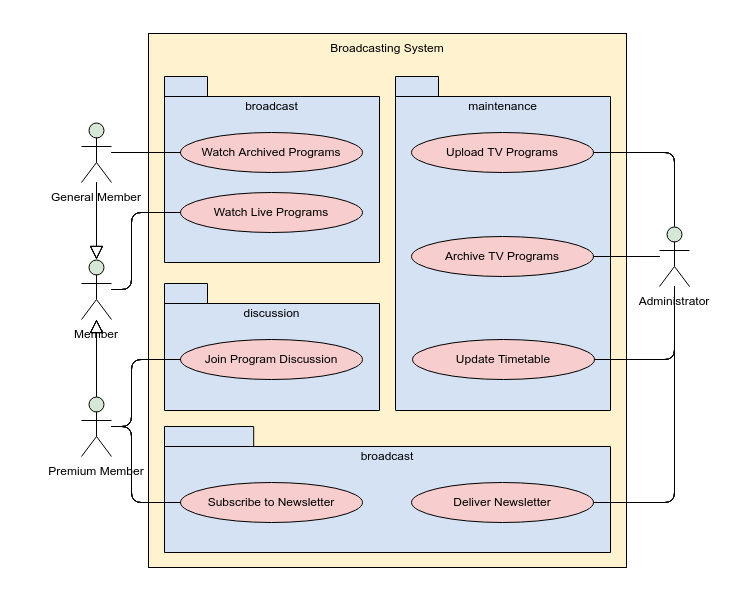
\includegraphics[scale=0.5]{Book-SSW565/png/UML Diagram.png} 
\end{figure}

\textbf{Broadcast System \gls{stakeholder}s:}
\begin{enumerate}
    \item System Administrator
    \item System Owner
    \item Viewer
\end{enumerate}

% Add a section and label it so that we can reference it later
\section{Applying Tactics of Availability \label{Section::Applying Tactics of Availability}}

\begin{longtable}{|l|p{12cm}|}
%\centering
\caption{\TableName{Quality Attribute: Availability} \TableLabel{QA: Availability} \label{Table::QA:Availability}}\\
    
    \hline
    \textbf{Portion} & \textbf{Possible Values}\\
    \hline 
    \endfirsthead

    \multicolumn{2}{c}{\tablename\ \thetable\ -- \textit{Continued from previous page}}\\
    \hline
    \textbf{Portion} & \textbf{Possible Values}\\
    \hline
    \endhead
    
    \multicolumn{2}{r}{\tablename\ \thetable\ -- \textit{Continued on next page}} \\
    \endfoot
    \endlastfoot

\gls{stakeholder} & System Administrator
\\ \hline

\gls{source} & Multiple requests, network failure, high traffic load
\\ \hline

\gls{stimulus} & Delay in response time, slow down system performance, unexpected server failure
\\ \hline

\gls{environment} & Normal Operation, System overloaded, network congestion, hardware failure
\\ \hline

\gls{artifact} & Load balancing system, redundant servers, monitoring tools
\\ \hline

\gls{response} & Detects, prevents, and recovers from faults by using tactics such as heartbeat monitoring, redundancy, load balancing, and fault recovery mechanisms
\\ \hline

\gls{responseMeasure} & System remains responsive within acceptable time limits, ensures minimal downtime by failing over to backup servers, retrying failed requests, and automatically adjusting resources (divide among multiple servers)
\\ \hline

\end{longtable}



\section{Applying Tactics of Performance\label{Section::Applying Tactics of Performance}}

\begin{longtable}{|l|p{12cm}|}
%\centering
\caption{\TableName{Quality Attribute: Performance} \TableLabel{QA: Performance} \label{Table::QA:Performance}}\\
    
    \hline
    \textbf{Portion} & \textbf{Possible Values}\\
    \hline 
    \endfirsthead

    \multicolumn{2}{c}{\tablename\ \thetable\ -- \textit{Continued from previous page}}\\
    \hline
    \textbf{Portion} & \textbf{Possible Values}\\
    \hline
    \endhead
    
    \multicolumn{2}{r}{\tablename\ \thetable\ -- \textit{Continued on next page}} \\
    \endfoot
    \endlastfoot

\gls{stakeholder} & System Administrator/Viewer
\\ \hline

\gls{source} & High incoming traffic, multiple concurrent viewer requests
\\ \hline

\gls{stimulus} & Increased latency, Increased response time, resource exhaustion
\\ \hline

\gls{environment} & Web application, cloud-based system, real-time processing, limited hardware resources
\\ \hline

\gls{artifact} & Application servers, databases, load balancers
\\ \hline

\gls{response} & Control resource demand (e.g., limit event response, prioritize events, reduce overhead) and Manage resources efficiently (e.g., introduce concurrency, schedule resources, maintain multiple copies of data, increase resources)
\\ \hline

\gls{responseMeasure} & Response generated within time constraints, optimized latency and throughput, and minimal resource wastage
\\ \hline

\end{longtable}